\section{问题描述}
本节我们先探究暴露模型中间结果带来的隐私泄露问题,然后定义本章所解决的三方协作的隐私保护机器学习问题。

\subsection{隐层表征的隐私泄露}
在拆分学习或部分密码学和拆分学习等其他方法混合的隐私保护机器学习框架中,模型的部分隐层表征会暴露~\cite{}。
%
这些研究对于安全性的论证往往基于中间表征的不可逆性质,也就是在没有辅助信息的情况下,从拆分表征恢复出原始的输入特征是不可能的。
%
比如考虑全连接神经网络的第一层表征$\bvec h=W \bvec x$,其中$W \in \mathbb R^{d_1 \times d_0}$是第一层的权重(这里忽略偏置项),$X \in \mathbb R^{d_0}$表示输入表征。
%
即使攻击者收集到了大量隐层表征$H = (\bvec h_1, \cdots, h_n)$,只需要隐层表征维度$d_1$小于输入特征维度$d_0$,线性方程组
\begin{equation}
\begin{cases}
    \bvec h_1 = W \bvec x_1 \\
    \cdots \\
    \bvec h_n = W \bvec x_n \\
\end{cases}
\end{equation}
就是有无穷多解的。
%
这是因为其已知量的个数 $nd_1$ 小于未知量的个数 $d_0d_1 + nd_0$。
%
尽管一些研究在特定条件下提出了对隐层表征进行攻击从而恢复训练特征的办法,但是这些方法往往需要一些额外信息,比如底部模型权重$W$,或是部分泄露的样本-表征对$(\bvec x_i, \bvec h_i)$。
%
接下来我们将说明,即使攻击者只搜集隐层表征,而没有模型的额外信息,依然存在隐私泄露的问题。

\textbf{样本间距离信息的隐私泄露}:
%
Johnson-Lindenstrauss定理~\cite{}告诉我们,对高维数据点的低维线性投影可以很大程度上保留数据点之间的距离关系。
%
也就是说,
\begin{equation}
    \Vert W \bvec x_1 - W \bvec x_2 \Vert_2 \approx c\Vert \bvec x_1 - \bvec x_2 \Vert,    
\end{equation}
其中$c$是一个和$W$的分布以及维度相关的常数。
%
考虑到神经网络的全连接层也可以视为一个随机线性投影,因此隐层表征之间的距离也可以反应原始输入特征之间的距离,从而使得整个数据集的拓扑结构信息被暴露。
%
以MNIST数据集为例,我们将784维的输入图片通过一个按照正态分布随机初始化的矩阵(类似于神经网络的权重初始化)投影到128维,然后对低维投影计算欧氏距离,找到最相似的样本,结果呈现在\autoref{fig:ss-perm:mnist-knn}中。
%

%
\begin{figure}[h!]
    \centering
    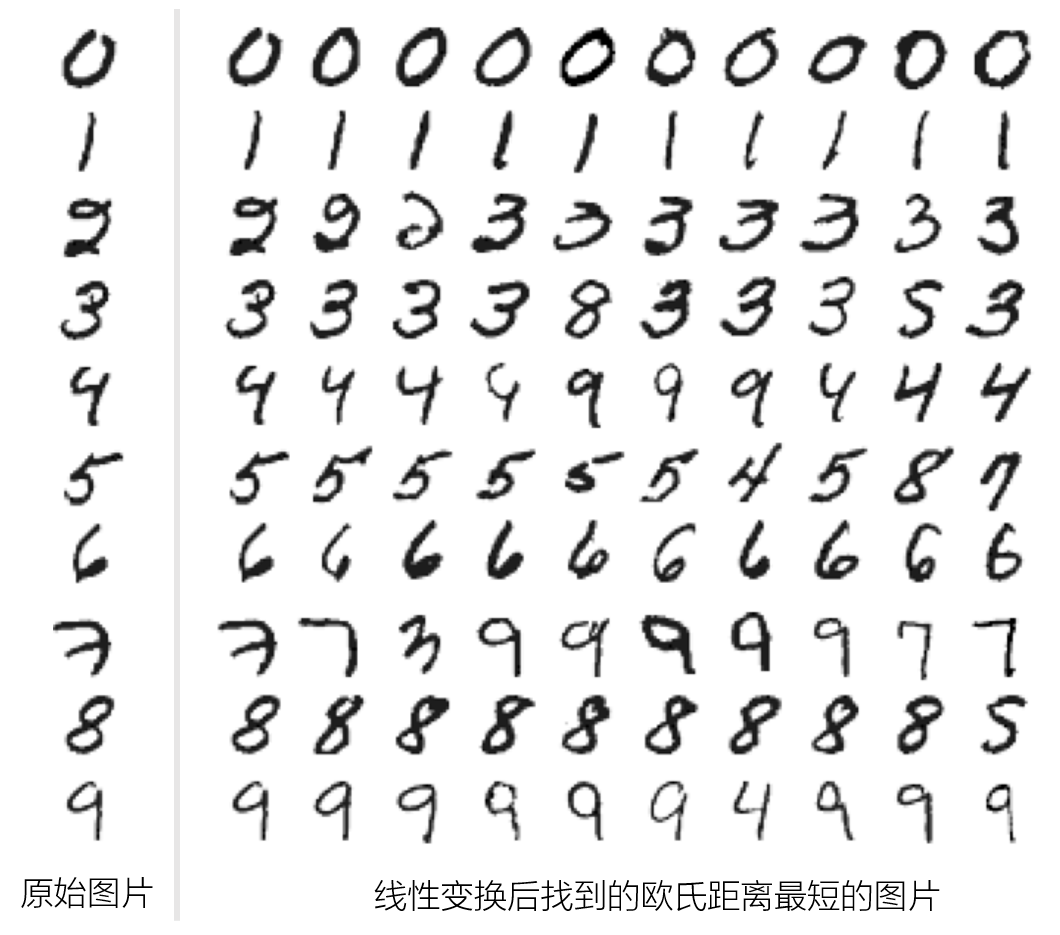
\includegraphics[width=0.66\linewidth]{Z_Resources/ss-perm_mnist-knn}
    \caption{通过对比低维投影得到的最相似样本}
    \label{fig:ss-perm:mnist-knn}
\end{figure}
%
可以看出,低维的投影相似的图片,其原始图片也几乎相似。
%
因此,攻击者可以通过分析隐层表征,得到特征拥有方的数据分布、数据之间的关系,乃至数据分布随着时间变化的变化等信息。
%
以疫情防控期间的口罩检测为例,假设某公司A采用了某公司B的“口罩检测”模型来判断员工是否按照规定佩戴了口罩,并采用拆分学习(或其他需要发送中间表征给公司B的方式)在公司内部监控摄像头的控制中心进行了模型部署。
%
公司B可以仅仅通过分析中间表征,而无需其他任何复杂的攻击操作,来判断公司A的员工出现状况。
若某一天公司A传输的中间表征的相似度与之前的中间表征的相似度降低,则可以判断公司A出现了较大的人事变动情况。
%
这显然对公司A的隐私信息造成了严重泄露。


\textbf{隐层表征的重用攻击}:
在纵向联邦学习开始前,各参与方需要进行样本对齐操作,即按照统一的样本ID对各参与方数据库中的样本进行统一,保证在训练中各方采用的是相同的样本。
%
因此,在纵向联邦学习过程中,某一个恶意的参与方也可以将样本的隐层表征信息记录下来,并对这些进行滥用。
%
比如某电商公司A为了训练更好的推荐系统,与某社交平台B达成协议,让社交平台B提供一部分用户数据并且以纵向联邦的方式进行训练。
两者采用用户的手机号作为ID进行样本对齐。
%
在训练过程中,A公司可以存储隐层表征信息。
%
训练完成后,A公司可以将这些隐层表征信息,连同对应的手机号售卖给其他公司。
%
虽然这些隐层表征信息主要是通过B公司的数据以及底部模型产生的,但是在拆分学习的场景下,B公司并没有有效的技术手段检测或防止A公司对其滥用的行为。
%
因此,这种隐层表征的重复利用攻击也对拆分学习的安全性带来了不利影响。

综上所述,使用拆分学习或是其他暴露中间结果的隐私保护机器学习方法,必然要面对中间结果与输入特征的关联性以及中间结果可能被再次利用的问题。


\subsection{本文问题定义}
本文考虑如下的隐私保护机器学习问题。
两方$P_0, p_1$分别持有部分数据$X$和模型参数$\Theta$,并且要进行模型的推断或训练,具体如下:
\begin{enumerate}
    \item 模型推断:计算 $Y = f(X; \Theta)$,其中$f$表示模型的推断函数,是公开的。要求在推断过程中,模型参数$\Theta$和各方数据$X$,以及其他中间结果尽可能不暴露,$Y$只暴露给设定的结果获取方,可能是$P_0$或$P_1$,也可以是其他方;
    \item 模型训练:计算 $\Theta' = g(X; \Theta)$,其中$g$表示模型的训练函数,比如对于梯度下降法,$g(X;\Theta) = \Theta - \alpha \partial L(X;\Theta) / \Theta$,其中$L$表示损失函数,$\alpha$是学习率。
    要求在训练过程中,模型参数$\Theta, \Theta'$,各方数据$X$,以及其他中间结果尽可能不暴露。
\end{enumerate}

在上述的隐私保护机器学习过程中,我们新增一个第三方$P_2$,其自身不带任何模型参数或数据,仅仅为$P_0$和$P_1$的计算提供辅助作用。
此外,我们假设各个参与方在执行特定的算法(协议)时,会遵守协议进行计算,但是其可能尽可能地利用其在执行协议中接收到的信息来获取其他参与方的隐私数据。
同时,任何参与方之间不会通过共谋(Collusion)来获取其他参与方的数据。
%
这个设定在密码学中被称为半可信安全性(Semi-Honest Security)设定或诚实但好奇(Honest-but-Curious)设定,在许多隐私保护机器学习算法的设计中被采用~\cite{}。